% !TEX TS-program = pdflatex
% !TEX encoding = UTF-8 Unicode
% !TEX ROOT = ../../main.tex

\section{Heidelberg in Flammen} %Bild von Heidelberg marketing oder privat

\begin{wrapfigure}{r}{0.5\textwidth}
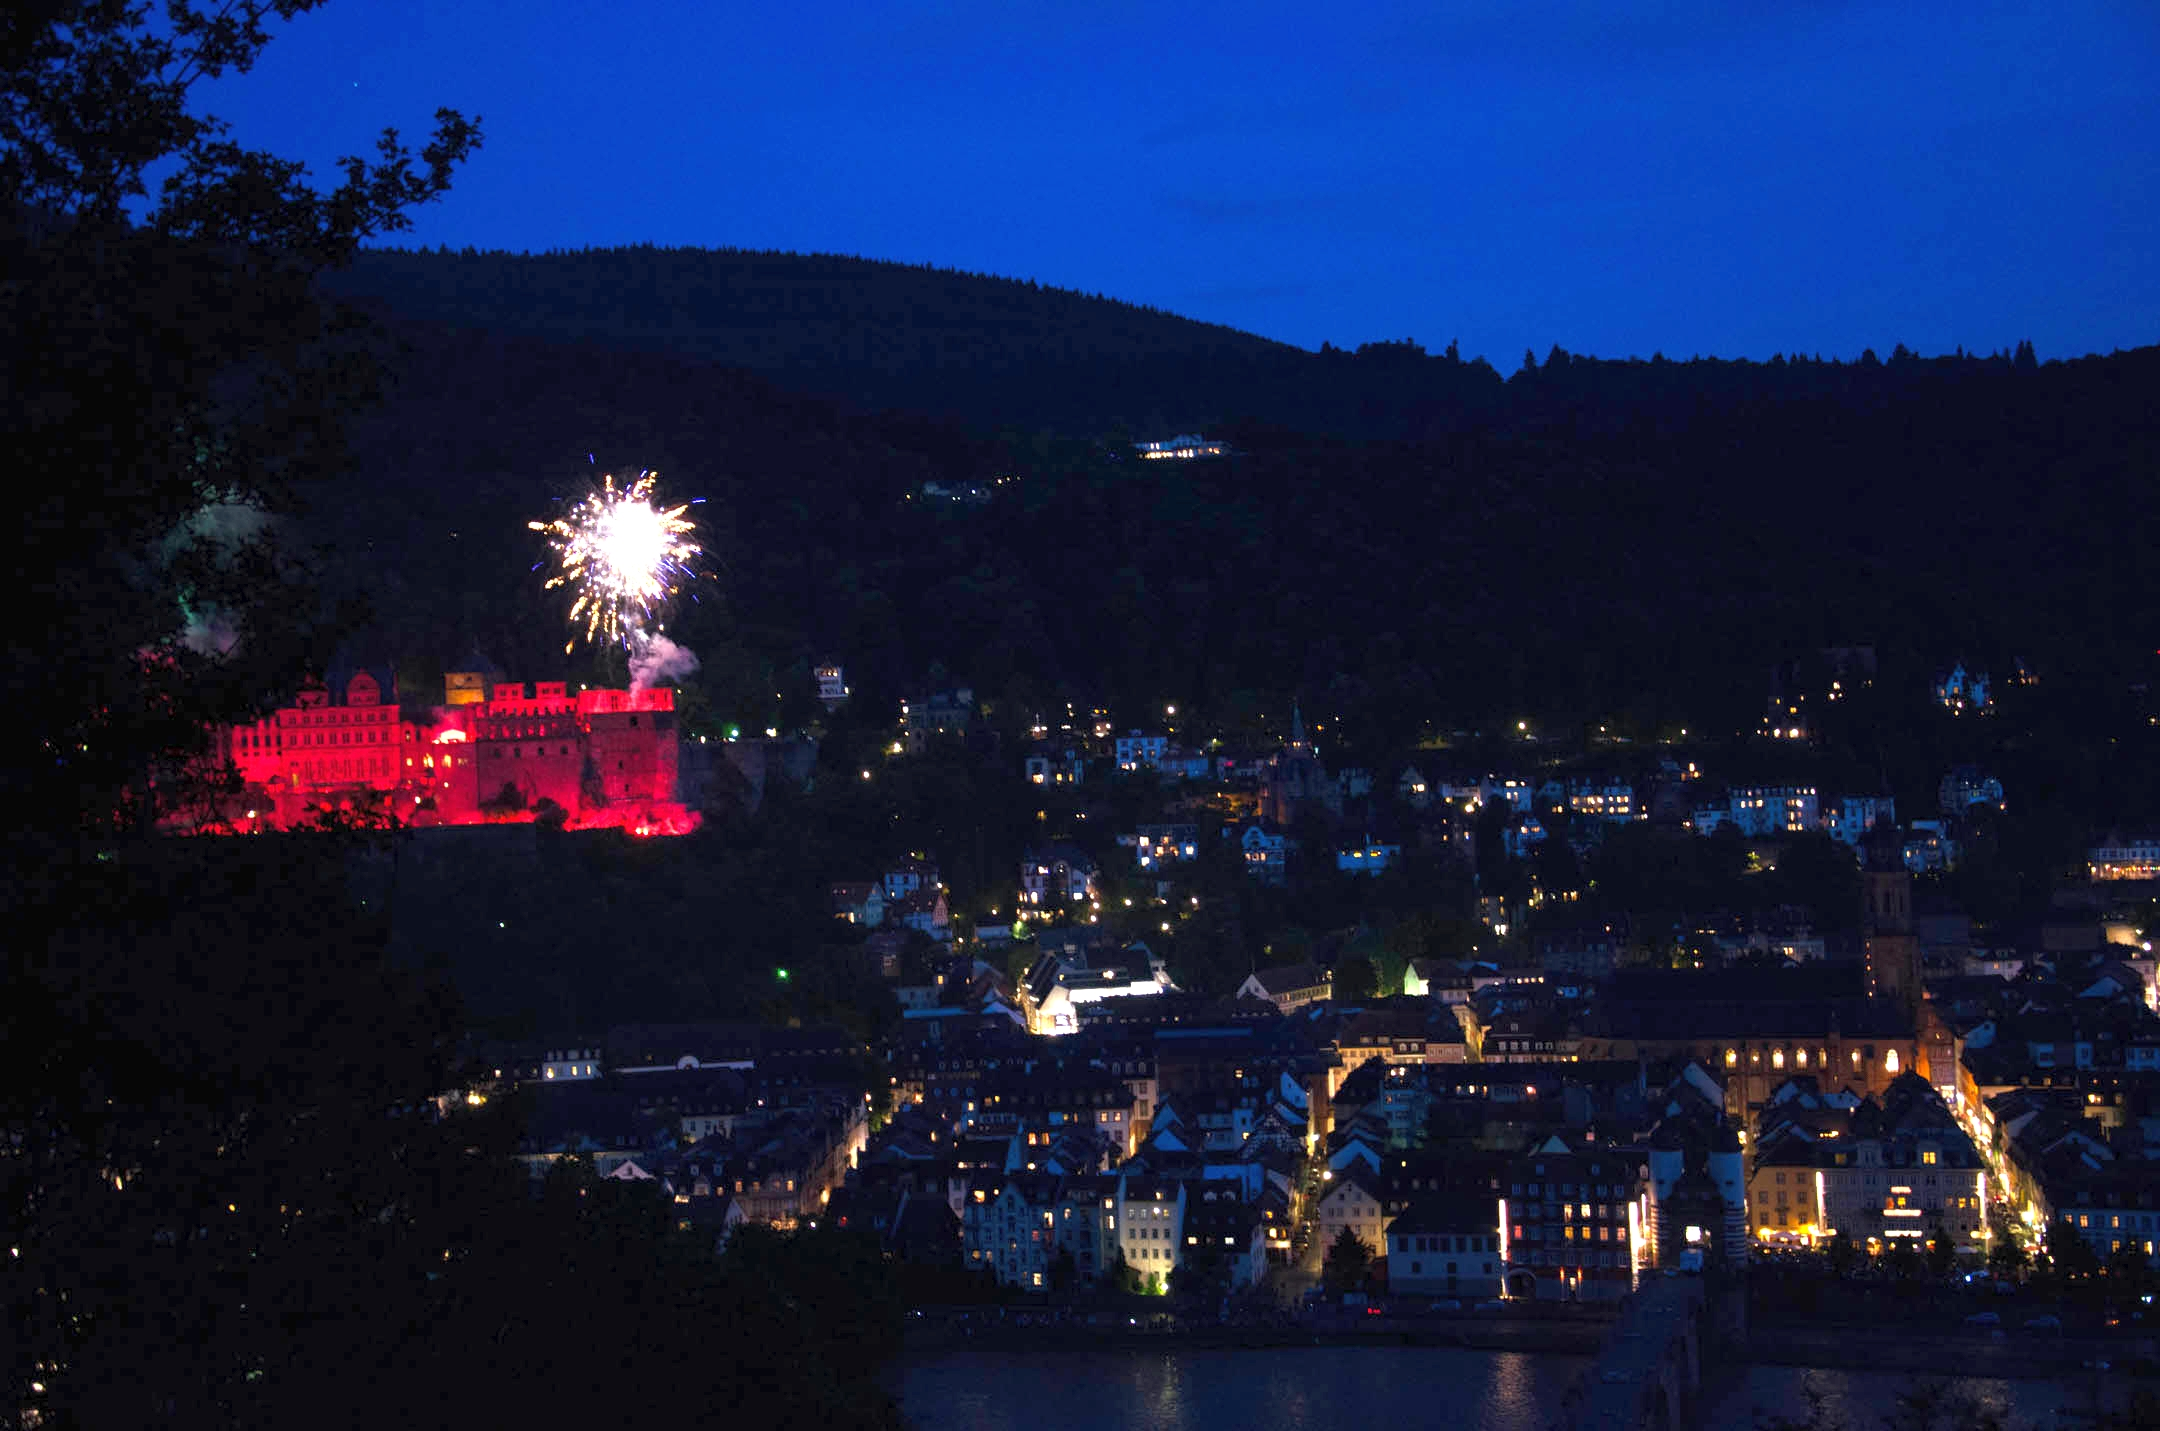
\includegraphics[trim= 10 150 400 120, clip, width=\linewidth]{Schlossbeleuchtung.jpg}
\end{wrapfigure}
Wir haben das Glück, dass just am Samstagabend der ZaPF zum ersten Mal im Jahr 2018 die mythische Heidelberger Schlossbeleuchtung stattfinden wird.

Dreimal im Sommer werden sowohl Alteingessenene als auch Neu--Heidelberger in ihren Bann gezogen um die Altstadt und die Schlossruine in ungewöhnlichen Farben erblicken zu dürfen.

Ganz so romantisch wie das Rot der bengalischen Feuer über dem Schloss dürfte der Anblick auf das niederbrennende Heidelberg 1693 allerdings nicht gewesen sein. Nach dem ersten Teil der Show am Schloss beginnt das von der Alten Brücke startende Feuerwerk. 

Die Schlossbeleuchtung findet \textbf{Samstag Abend ab ca. 22:15 Uhr} statt. Empfohlene Aussichtspunkte sind der Schlossgarten und insbesondere der Philosophenweg. Der Treffpunkt, um uns das Spektakel gemeinsam anzuschauen, wird rechtzeitig über die Kommunikationskanäle der ZaPF bekannt gegeben.
%\begin{wrapfigure}
%\centering
%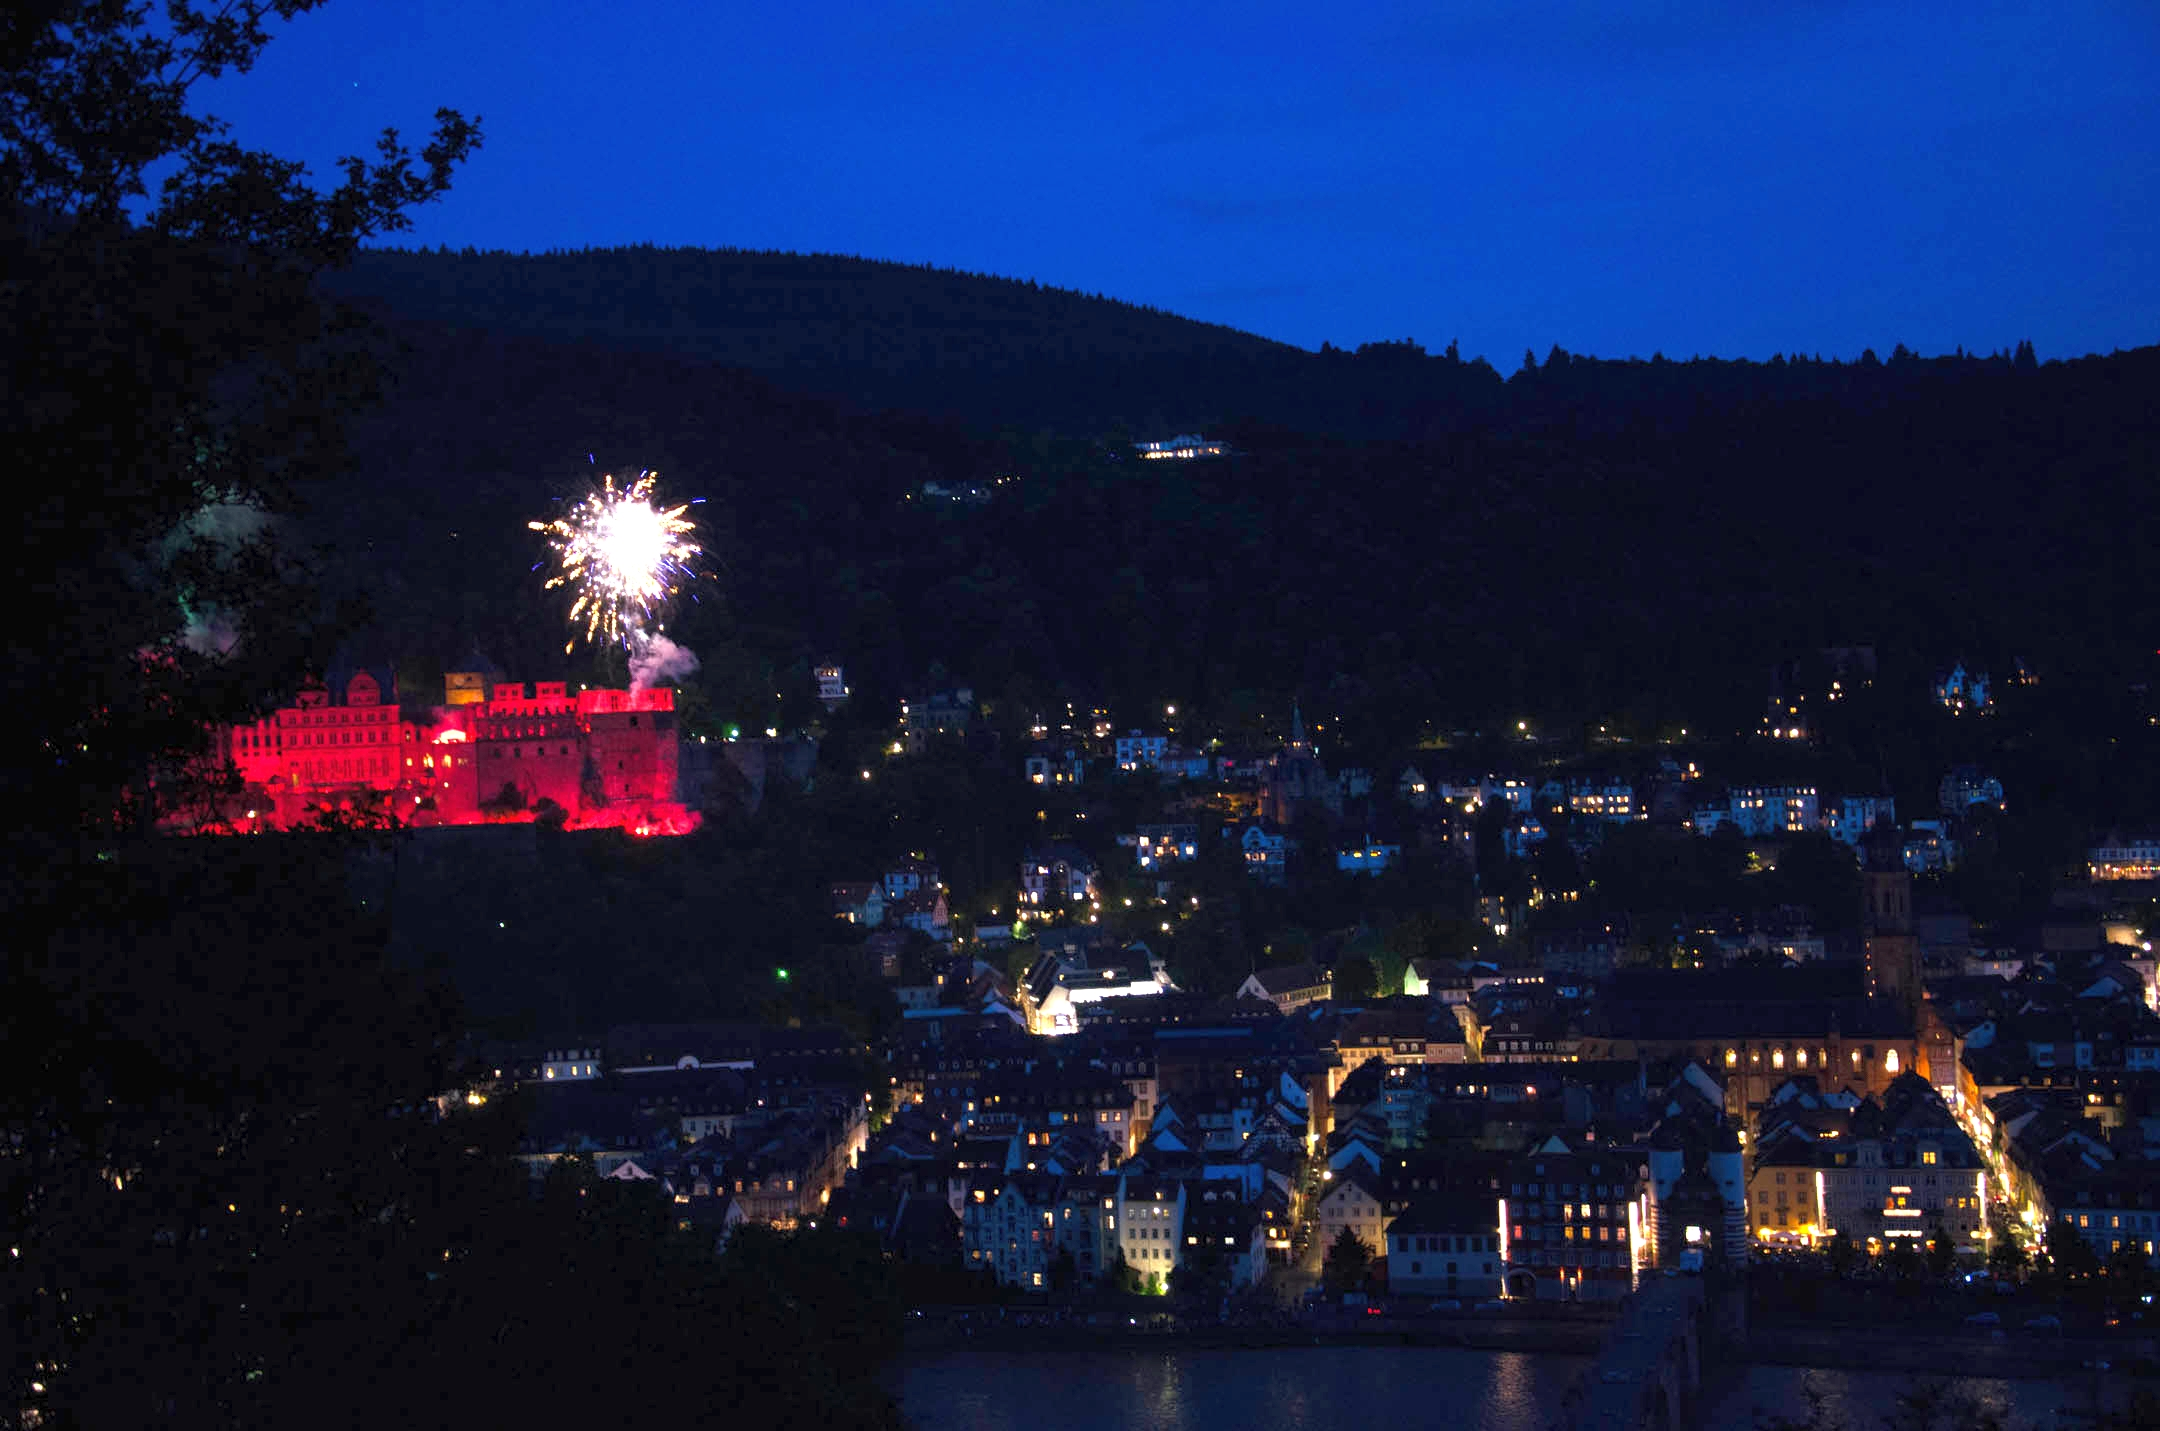
\includegraphics[trim= 10 100 400 100, clip, width=0.7\textwidth]{Schlossbeleuchtung.jpg}
%\end{wrapfigure}
